\documentclass[14pt,aspectratio=1610]{beamer}
\usepackage[utf8]{inputenc}
\usepackage[ngerman]{babel}
\uselanguage{ngerman}
\languagepath{ngerman}
\usetheme{simple}
\usecolortheme{whiteonblack}
\usepackage{array}
\usepackage{aurl}
\daurl{meta}{http://www.snik.eu/ontology/meta/}
\daurl{ob}{http://www.snik.eu/ontology/ob/}
\daurl{bb}{http://www.snik.eu/ontology/bb/}
\usepackage{url}
\usepackage{graphicx}
\usepackage{csquotes}
\usepackage{amssymb}
\usepackage{pifont}
\newcommand{\xmark}{\ding{55}}%
\newcolumntype{H}{>{\setbox0=\hbox\bgroup}c<{\egroup}@{}} % comment out columns
\date{5. Oktober 2016}
\author{\texorpdfstring{Konrad Höffner\newline\url{konrad.hoeffner@imise.uni-leipzig.de}}{Konrad Höffner}}
\title{SNIK Ontologie---Lehre und Implementierung}
\subtitle{mit nachträglichen Anmerkungen vom 10. Oktober 2016}
\begin{document}
\begin{frame}
\titlepage
\end{frame}

\begin{frame}{Vorstellung}
\only<1>
{
\begin{itemize}
\item Konrad Höffner
\item Studium Diplominformatik an Uni Leipzig
\item Doktorand der Informatik beim AKSW, Uni Leipzig/InfAI
\item Thema \enquote{Question Answering auf RDF Data Cubes}
\item bei IMISE und im SNIK Projekt seit Juli
\item kein Vorwissen über Medizin aber viel praktische Erfahrung mit Semantic Web-Technologien
\end{itemize}
}
\only<2>
{
\begin{itemize}
\item Visualisierung, Implementierung, Serialisierung
\item Qualitätssicherung
\item Aufsetzen von Services
\vspace{1em}
\item Raum 227, Tel. (0341)97-16363
\item \href{mailto://konrad.hoeffner@imise.uni-leipzig.de}{konrad.hoeffner@imise.uni-leipzig.de}
\item \url{https://github.com/KonradHoeffner/latex/tree/master/beamer/2016/snik-projekttreffen}
\end{itemize}
}
\end{frame}

\section{Einsatz in der Lehre}

\begin{frame}{}
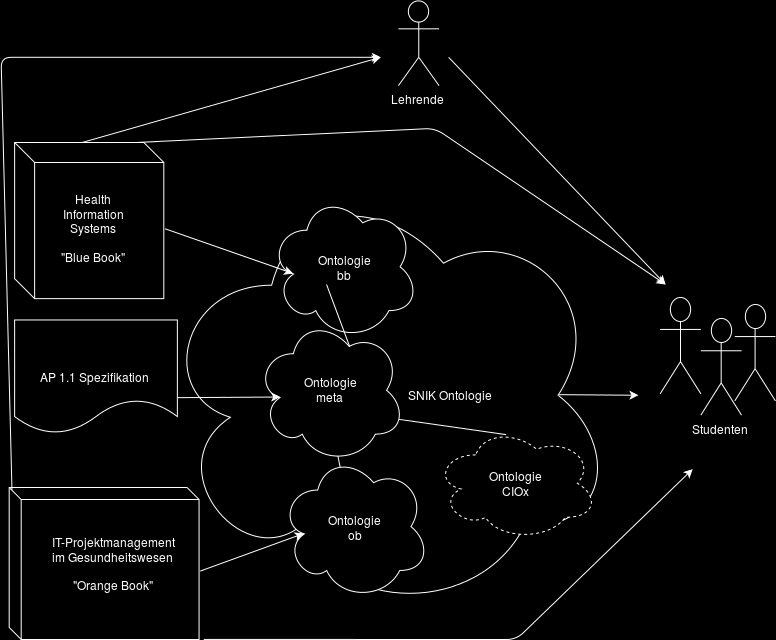
\includegraphics[width=\textwidth,height=0.9\textheight,keepaspectratio]{img/lehre.png}
\end{frame}

\begin{frame}{Ziele}
\begin{itemize}
\item modelliertes Wissen vermitteln, zusätzlich zu Lehrbüchern, Vorlesungen und Übungen
\item Exploration 
\item Erstellen von Übungsaufgaben
\item Semantic Web nur Mittel zum Zweck, so viel Zeit wie möglich für Gesundheitsinformationssysteme 
\end{itemize}
\end{frame}

\begin{frame}{Problem}
\begin{itemize}
\item Studenten sind zwar (Medizin-)Informatiker, haben aber nicht zwangsweise die Semantic Web Vorlesungen von Prof. Fähnrich besucht
\item $\rightarrow$ kein Vorwissen in SPARQL und RDF-Serialisierungsformaten vorauszusetzen
\item Protégé kein intuitiver Gesamtüberblick, getestete Graphplugins skalieren nicht
\item Lösung: Eigenentwicklung einer Visualisierung unter Verwendung ausgereifter Bibliotheken
\end{itemize}
\end{frame}

\begin{frame}{\url{http://www.snik.eu/(p)graph/}}
\begin{itemize}
\item Öffentliche alte Version (wird aktualisiert) ohne CIOx \url{http://www.snik.eu/graph/}
\item Passwortgeschützte neue Version mit CIOx \url{http://www.snik.eu/pgraph/}
\item CIOx-Ontologie enthält Betriebsinterna, Zugangsdaten nur auf sichere Art und Weise an Befugte Weitergeben! 
\end{itemize}
\end{frame}

\begin{frame}{}
\centering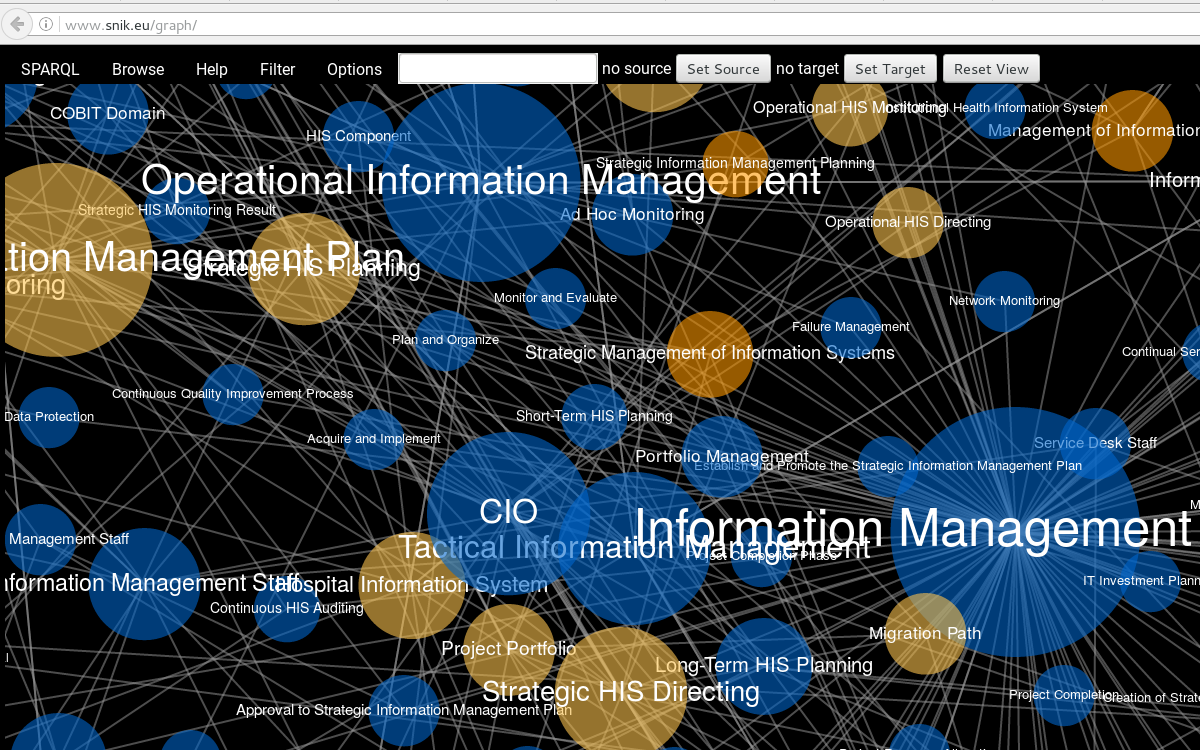
\includegraphics[width=1.05\textwidth,height=1.05\textheight,keepaspectratio]{img/browser.png}
\end{frame}

\begin{frame}{}
\centering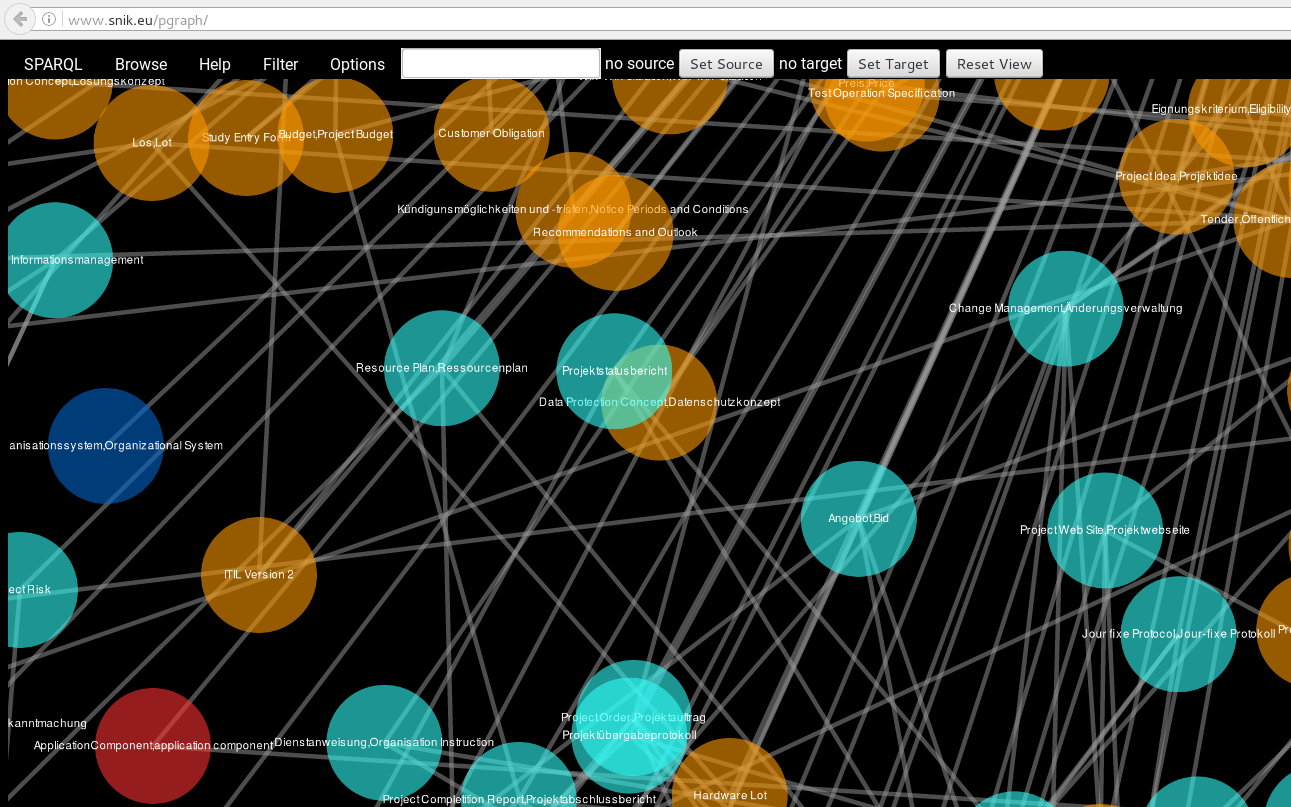
\includegraphics[width=1.05\textwidth,height=1.05\textheight,keepaspectratio]{img/pbrowser.png}
\end{frame}

\begin{frame}{Kürzester Weg}
\centering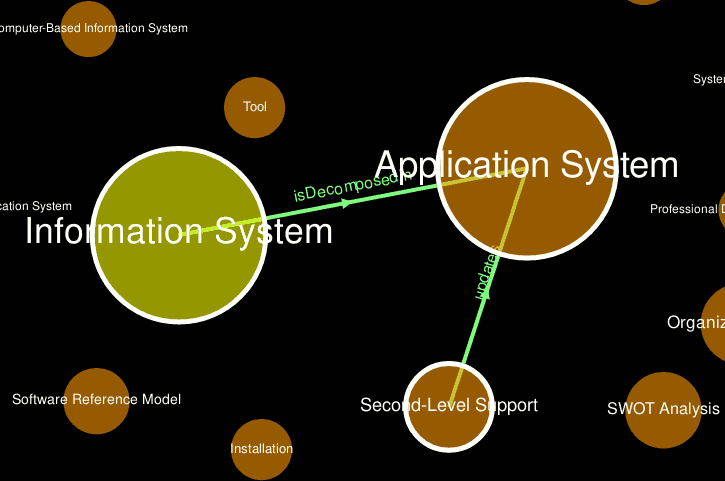
\includegraphics[width=\textwidth,height=\textheight,keepaspectratio]{img/shortestpath.png}
\end{frame}

\begin{frame}{Spiderworm}
\centering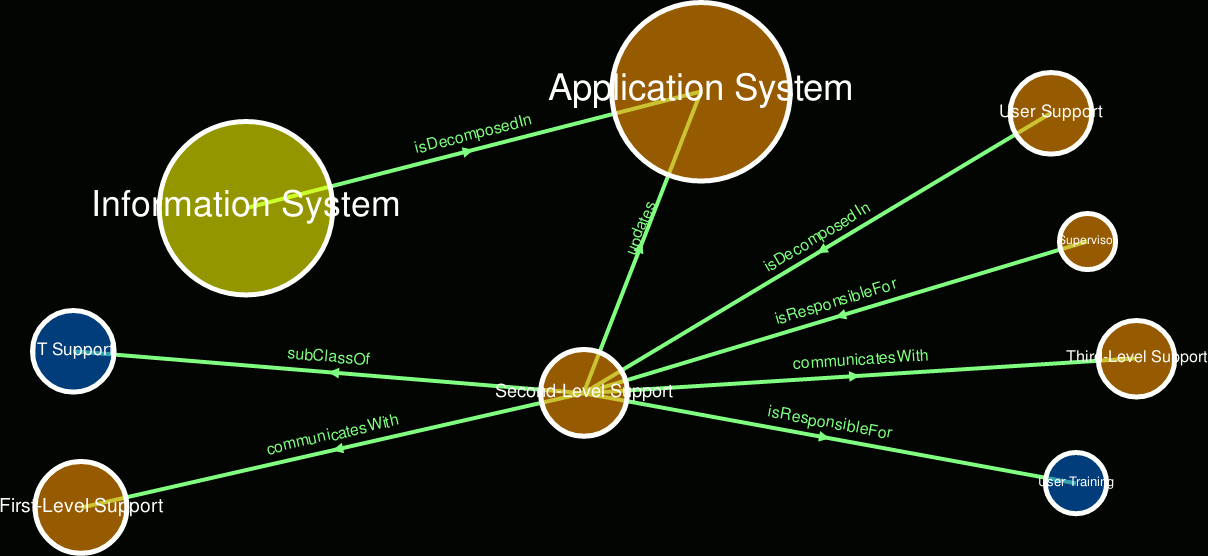
\includegraphics[width=\textwidth,height=\textheight,keepaspectratio]{img/spiderworm.png}
\end{frame}

\begin{frame}{Praktische Vorführung}
\begin{itemize}
\item Kürzester Weg und Spiderworm
\item Suche
\item Filterung
\item Hilfe
\item Feedback
\item Browse
\end{itemize}
\end{frame}

\section{Implementierung}%********************************************************

\subsection{Modellierung und Serialisierung}%****************************


\begin{frame}{Modellierung und Serialisierung}
\begin{block}{Überblick}
\begin{tabular}{ll}
Ontologie	&Anzahl Tripel\\
meta	&244\\
bb	&35803\\
links-bb	&79\\
ciox	&1933\\
links-ciox	&29\\
ob	&25894\\
gesamt	&63982\\
\end{tabular}
\end{block}
\end{frame}

\begin{frame}{Modellierung und Serialisierung}
\begin{block}{Überblick\footnote{Untere Schranken, noch nicht alle \aurl{meta}{subTop}-Beziehungen modelliert.}}
\begin{tabular}{ll}
Oberklasse	&Anzahl\\
\aurl{meta}{Role}	&79\\
\aurl{meta}{Function}	&154\\
\aurl{meta}{EntityType}	&1395\\
\end{tabular}
\end{block}
\end{frame}

\begin{frame}{Modellierung und Serialisierung}
\begin{block}{Ausgangssituation}
\begin{itemize}
\item SNIK-Ontologien bb, ob und ciox wurden mit Protégé bearbeitet und als RDF/XML serialisiert
\item bei Änderungen mussten andere Personen informiert und mit aktualisierten Dateien versorgt werden 
\item $\rightarrow$ schwierige Kooperation 
\end{itemize}
\end{block}
\end{frame}

\begin{frame}{Modellierung und Serialisierung}
\begin{block}{Lösung}
\begin{itemize}
\item Einsatz des Versionskontrollsystems git
\item RDF/XML-Serialisierung mit Texteditor bearbeitet
\item gleichzeitige Änderungen möglich, Konflikte durch git merge-Mechanismus beheben
\item Rückkehr zu jedem früheren Zeitpunkt möglich
\item durch reguläre Ausdrucke gleichzeitige Änderungen an hunderten Entitäten gleichzeitig möglich
\item Änderungen benötigen Kenntnisse in RDF/XML und git
\item wenn großflächige syntaktische Änderungen fertig, Rückkehr zur Protégé möglich
\end{itemize}
\end{block}
\end{frame}

\begin{frame}{Modellierung und Serialisierung}
\begin{block}{Modellierungsprinzipien}
\begin{itemize}
\item Verwendung existierender Vokabulare
\item Konsistenz: gleiche Eigenschaften auf gleiche Weise modellieren
\item Zusammenfassen von gleichen Werten zu mehrfach genutzten Objekten, ähnlich Normalform bei Datenbanken, reduziert Inkonsistenzen, Arbeitsaufwand und Fehleranfälligkeit (Bsp.: Lehrbuchquelle)
\item Bevorzugen von Object Properties gegenüber Data Type Properties
\end{itemize}
\end{block}
\end{frame}

\begin{frame}{Modellierung und Serialisierung}
\begin{block}{Prefixe und Vokabulare}
\small
{
\begin{tabular}{l>{\footnotesize}ll}
Ontologie	&Prefix						&Inhalt\\
meta		&\url{http://www.snik.eu/ontology/meta}		&SNIK Meta-Ontologie\\
bb		&\url{http://www.snik.eu/ontology/bb}		&SNIK Blaues Buch\\
ob		&\url{http://www.snik.eu/ontology/ob}		&SNIK Oranges Buch\\
ciox		&\url{http://www.snik.eu/ontology/meta}		&SNIK CIOx Interviews\\
ov		&\url{http://open.vocab.org/terms/}		&Ontologiedefinition\\
%vann		&\url{http://purl.org/vocab/vann/}	&\\%too little usage
skos		&\url{http://www.w3.org/2004/02/skos/core\#}	&Interlinks, Definitionen\\
dc		&\url{http://purl.org/dc/terms}			&Metadaten\\
bibo		&\url{http://purl.org/ontology/bibo/}		&Bibliographie\\
%		&\url{}					&\\
\end{tabular}
}
~\\
Dazu Standardvokabulare RDF, RDFS, OWL.
\end{block}
\end{frame}

\begin{frame}{Modellierung und Serialisierung}
\begin{block}{Anwendung der Prinzipien}
\begin{itemize}
\item konsequente Anwendung der Prinzipien zieht große Zahl an Änderungen nach sich
\item in 3 Monaten: 31000 hinzugefügte, 28000 entfernte Zeilen
\item teilweise automatisierbar, teilweise Entscheidung bei jedem Fall nötig
\item Gartenmetapher: es ist immer etwas zu tun
\end{itemize}
\end{block}
\end{frame}

\begin{frame}[fragile]{Modellierung und Serialisierung}
\begin{block}{Anwendung der Prinzipien: Beispiel Synonyme}
\begin{itemize}
\only<1>
{
\item Synonyme sind mit \texttt{<Synonym>Text</Synonym>} modelliert 
\item Problem 1a: Benutzung des leeren Präfixes führt bei jeder Teilontologie zu anderer URI (\aurl{ob}{Synonym}, \aurl{bb}{Synonym}, $\ldots$) 
\item Problem 1b: Synonym ist nicht definiert, daher genaue Semantik unbekannt, wird auch anderswo nicht verwendet
}
\only<2>
{
\item Typische Lösung: Identifizieren und Verwenden eines existierenden Vokabulars
\item Also: Ersetzen von \texttt{Synonym} durch \texttt{\aurl{skos}{altLabel}}
\item Problem 2a: Wie entscheidet sich, welches label \aurl{rdfs}{label} und welches \aurl{skos}{altLabel} wird? Existierende Daten inkonsistent z.B. bei Abkürzungen. 
\item Problem 2b: Language tags fehlen, entweder "de" oder "en".
\item $\rightarrow$ manuelles Entscheiden in > 500 Fällen, Abkürzungen immer \aurl{skos}{altLabel}
}
\end{itemize}
\end{block}
\end{frame}

\begin{frame}[fragile]{Modellierung und Serialisierung}
\begin{block}{Anwendung der Prinzipien: Beispiel Transitivität}
\begin{itemize}
\only<1>
{
\item Materialisierung von transitiven Properties wie \aurl{rdfs}{subClassOf}
\item $A \subseteq B \subseteq C \rightarrow A \subseteq C$
\item Diese Tripel können inferiert werden, Virtuoso und die Cytoscape.js unterstützen dies aber nicht.
\item Materialisierte Tripel können von anderen nicht unterschieden werden und machen Visualisierung unübersichtlich.
}
\only<2>
{
\item Entscheidung: Nichts materialisieren, alles materialisieren oder nur zweitoberste Klasse (\aurl{meta}{Role}/Function/EntityType) materialisieren? (oberste ist \aurl{meta}{Top})
\item Anfangszustand: Teilweise nichts materialisiert, teilweise zweitoberste Klasse materialisiert.
\item Entscheidung: Oberste Klasse mit neuer Property, \aurl{meta}{subTopClass} angegeben, in Visualisierung nicht angezeigt
}
\end{itemize}
\end{block}
\end{frame}

\begin{frame}{Modellierung und Serialisierung}
\begin{block}{Ausblick}
\begin{itemize}
\item Fertigstellung großflächiger syntaktische Änderungen
\item Kooperative punktuelle semantische Änderungen durch Domänenexperten
\item siehe Abschnitt Qualitätssicherung 
\end{itemize}
\end{block}
\end{frame}

\subsection{Visualisierung}%****************************

\begin{frame}{Visualisierung}
\begin{block}{Anforderungen}
\begin{itemize}
\item performant bei mehreren tausend Knoten und Kanten 
\item keine Installation nötig
\item geringer Implementationsaufwand
\item Suchfunktion
\item Filterung
\item Graphoperationen wie kürzeste Wege, Spiderworm
\end{itemize}
\end{block}
\end{frame}

\begin{frame}{Visualisierung}
\begin{block}{Designentscheidungen}
\begin{itemize}
\item Javascript $\rightarrow$ keine Installation nötig, immer verfügbar, kein Server nötig
\item Cytoscape.js performante Graphbibliothek mit genügend Funktionalität
\item SPARQL Endpunkt mit bif:contains-Index für schnelle Suche (future work: Lucene Index)
\item Pubby SPARQL Browser zur Detailansicht 
\end{itemize}
\end{block}
\end{frame}

\begin{frame}{Visualisierung}
\begin{block}{Datenbereitstellung}
\begin{itemize}
\item Cytoscape.js kann RDF nicht direkt verarbeiten, hat aber CSV import
\item Virtuoso SPARQL Endpunkt kann Ergebnisse als CSV-Dateien abspeichern
\item Ontologie nicht 1:1 abgebildet, z.B. Abflachen von OWL Restrictions 
\item CSV Dateien Cytoscape Desktop importieren, als JSON exportieren
\item JSON-Datei mit Cytoscape.js loaden
\end{itemize}
\end{block}
\end{frame}

\begin{frame}{Visualisierung}
\begin{block}{Suche mit bif:contains SPARQL Query}
\centering
\only<1>{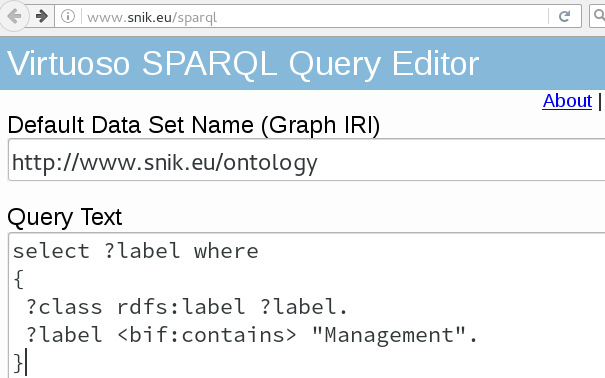
\includegraphics[width=\textwidth,height=0.7\textheight,keepaspectratio]{img/bifcontains-query.png}}
\only<2>{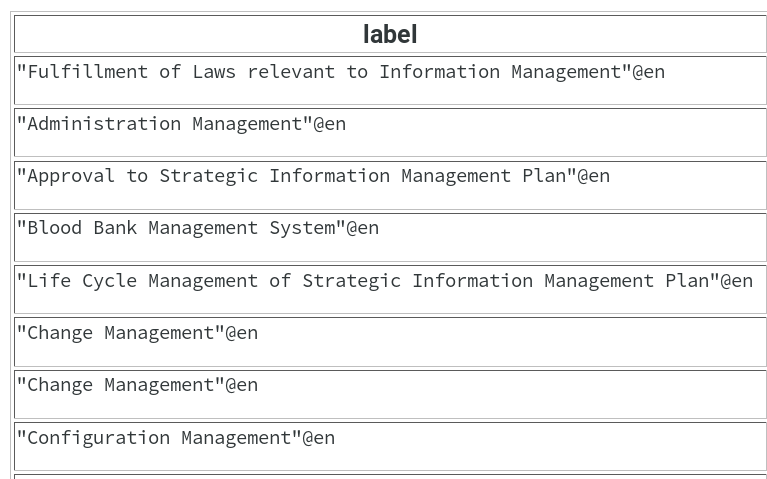
\includegraphics[width=\textwidth,height=0.7\textheight,keepaspectratio]{img/bifcontains-result.png}}
\end{block}
\end{frame}

\begin{frame}{Visualisierung}
\begin{block}{Ausblick}
\begin{itemize}
\item Suche von Phrasen statt Wörtern
\item Suche mit Synonymen und Schreibfehlern
\item z.B. durch Apache Lucene/SOLR index
\item Bugfixing
\item Wechsel von Pubby zu modernerem RDF browser
\item Export von Selektionen
\end{itemize}
\end{block}
\end{frame}

\subsection{Qualitätssicherung}%*******************************************

\begin{frame}{Qualitätssicherung}
\begin{block}{Ausgangspunkt: 5 Star Linked Data}
\begin{enumerate}
\item Daten sind im Web in irgendweinem Format verfügbar \checkmark{}
\item maschinenlesbare strukturierte Daten (z.B. kein PNG) \checkmark{}
\item nichtprorietäres Format (z.B. CSV, nicht Excel) \checkmark{}	
\item nach den offenen Standards des W3C publiziert (RDF and SPARQL) \checkmark{}
\item mit Links zu anderer Linked Data \checkmark (zwischen Teilontologien) / \xmark{} (außerhalb SNIK)
\end{enumerate}
\end{block}
\end{frame}

\begin{frame}{Qualitätssicherung}
\begin{block}{Dimensionen der Qualität}
\begin{itemize}
\item \href{Quality Assessment for Linked Data: A Survey}{http://www.semantic-web-journal.net/content/quality-assessment-linked-data-survey}, Meta-Studie von Amrapali Zaveri
\item 18 gemeinsame Dimensionen
\item teilweise subjektiv
\item aufwändig zu bestimmen, teilweise Crowdsourcing nötig
\end{itemize}
\end{block}
\end{frame}

\begin{frame}{Qualitätssicherung}
\begin{block}{Dimensionen der Qualität---Beispiele}
\begin{itemize}
\item Accessibility -- Serialisierte Dateien, SPARQL Endpunkt, im Browser aufrufbare URLs
\item Lizenzen -- bei Datenbanken nicht betrachtet aber bei Linked Data notwendig 
\item Interlinking -- Verknüpfungen von und zu anderen Datensets 
\item Performance -- Latenzzeit, Skalierbarkeit
\item Understandability, Completeness, Relevanz, $\ldots$
\end{itemize}
\end{block}
\end{frame}

\begin{frame}{Qualitätssicherung}
\begin{block}{Designierte Manuelle Korrektur}
\begin{itemize}
\item semantische Korrektheit von Fakten benötigt manuellen Input
\item serielles Durcharbeiten der serialisierten Ontologien beschränkt Personen auf Schnittmenge von Semantic-Web-Experten und Domänenexperten
\item besser: zufällige Stichproben von Fakten
\item manuell ausgezeichnet als korrekt, falsch oder ungewiss 
\end{itemize}
\end{block}
\end{frame}

\begin{frame}{Qualitätssicherung}
\begin{block}{Designierte Manuelle Korrektur}
\begin{itemize}
\item Korrektur kann in beliebig großen Arbeitsabschnitten erfolgen
\item bei Überschneidung inter-rater-agreement
\item Triple Checkmate Tool von AKSW 
\end{itemize}
\end{block}
\end{frame}

\begin{frame}{Qualitätssicherung}
\begin{block}{Feedback von Visualisierung}
\begin{itemize}
\item wenn Fehler bemerkt werden, kann Ticket erstellt werden
\item \url{https://bitbucket.org/imise/snik-ontology/issues}
\item Feedback für Visualisierung und Ontologie getrennt
\item (wenn Internet funktioniert) Vorführung 
\end{itemize}
\end{block}
\end{frame}

\begin{frame}{Cytoscape Desktop}
\centering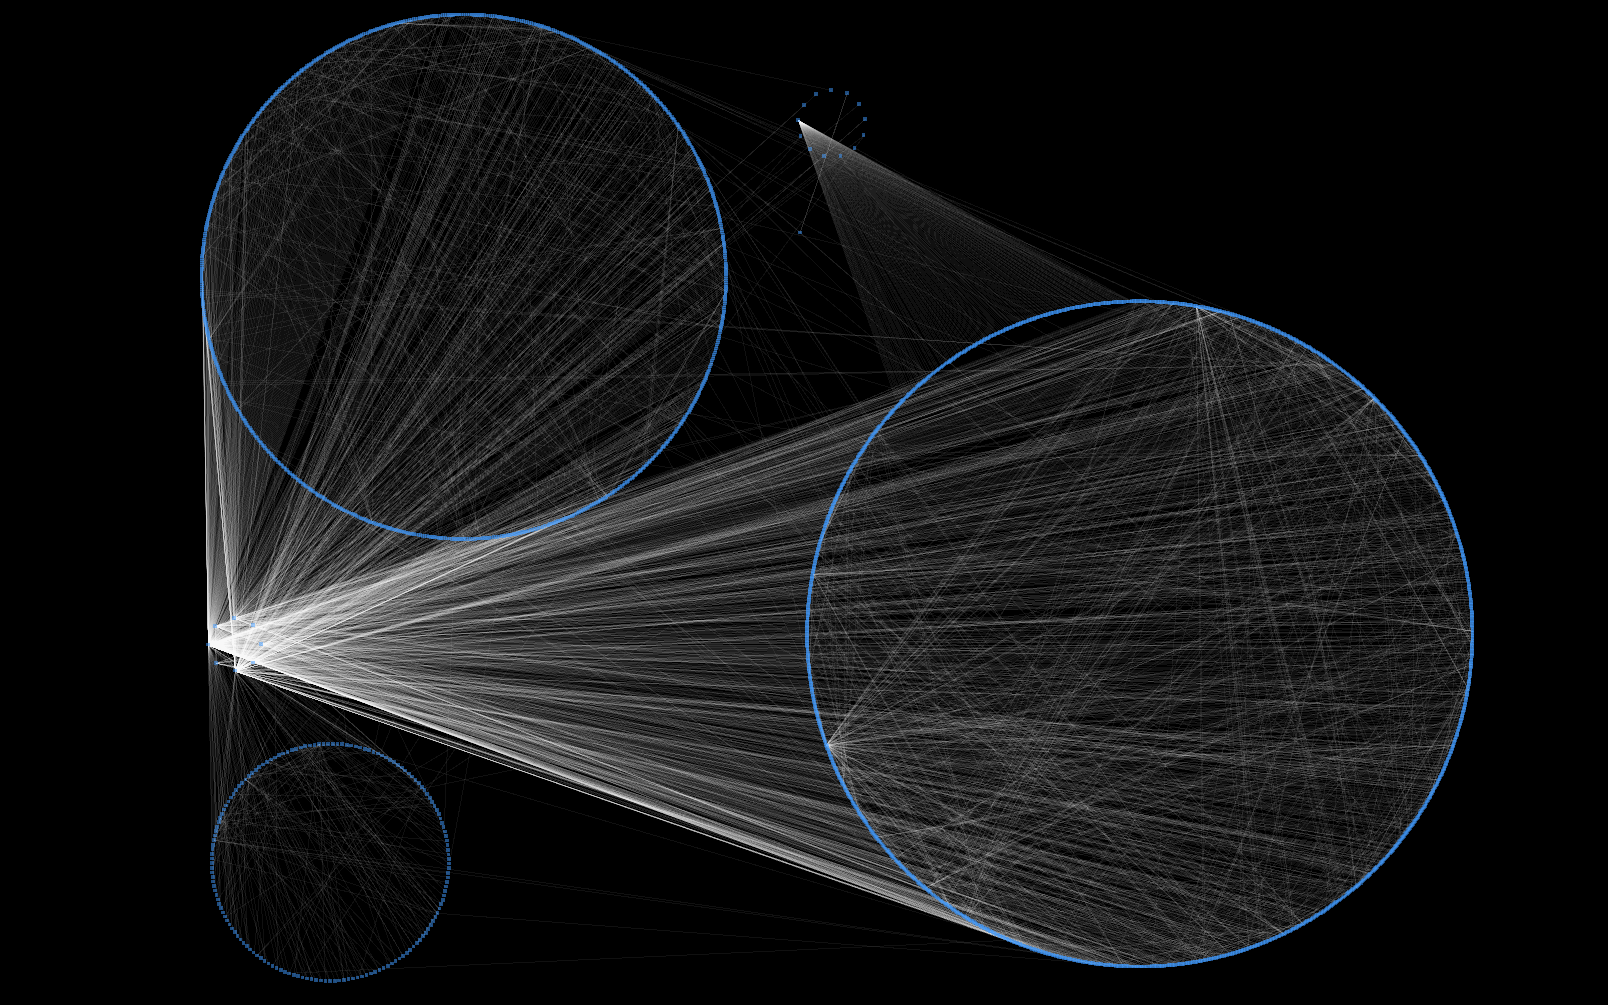
\includegraphics[width=\textwidth,height=\textheight,keepaspectratio]{img/types_classrelations.png}
\end{frame}

\begin{frame}{Cytoscape Desktop}
\centering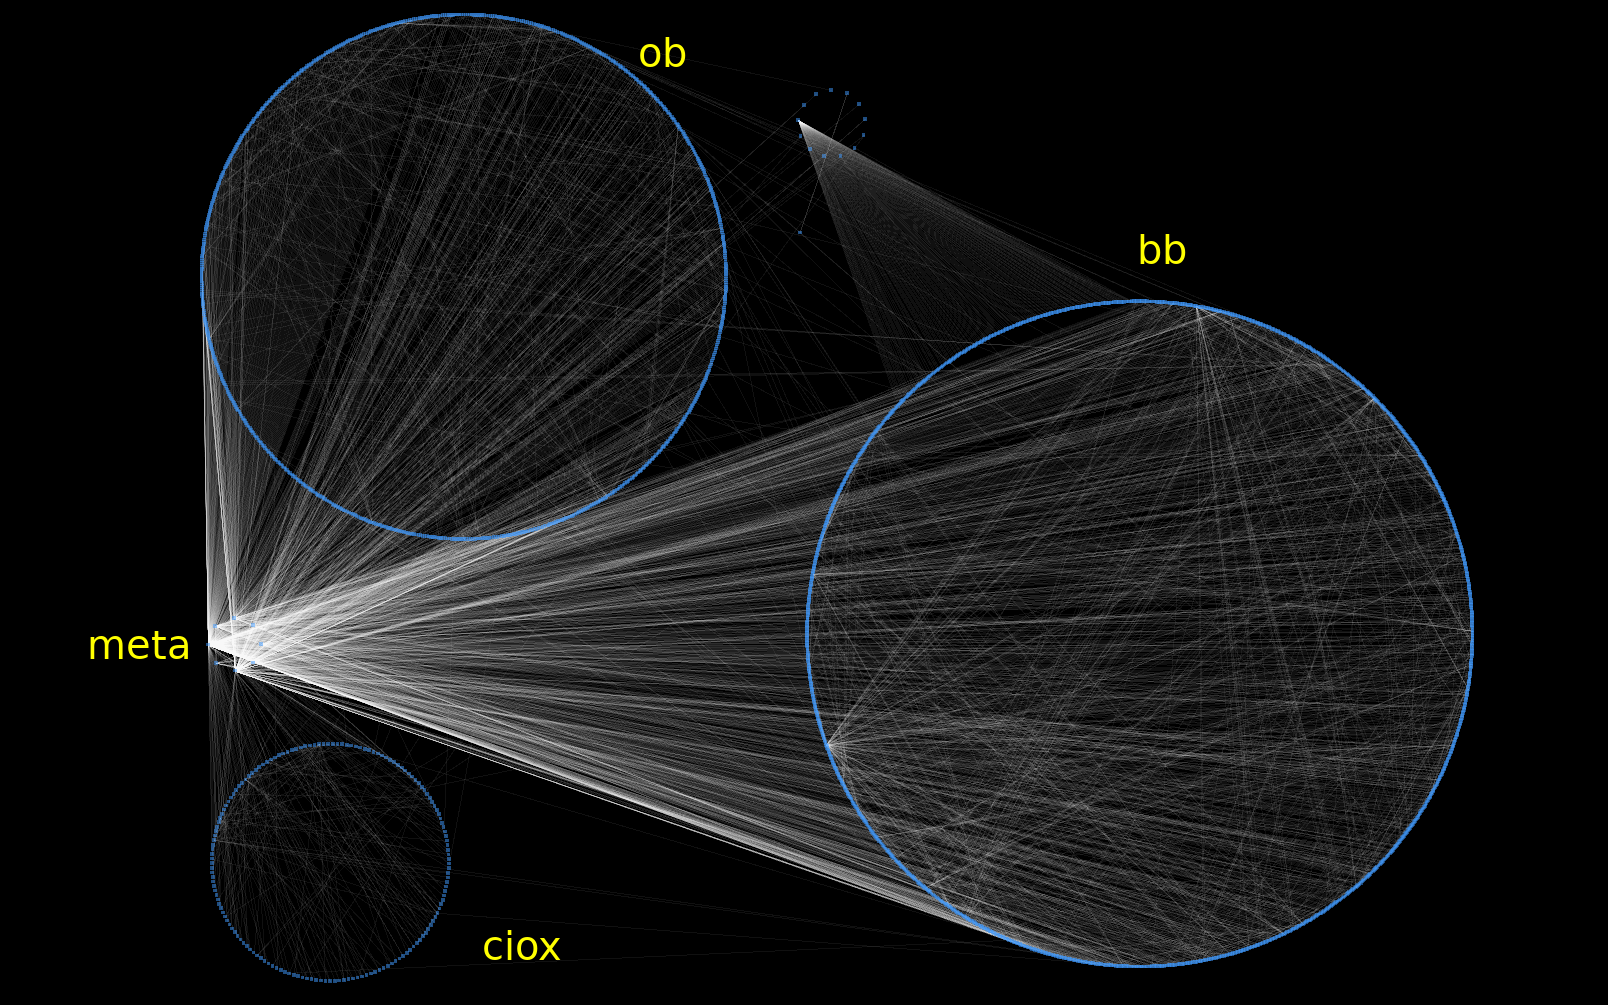
\includegraphics[width=\textwidth,height=\textheight,keepaspectratio]{img/types_classrelations_labelled.png}
\end{frame}

\begin{frame}{Cytoscape Desktop}
\centering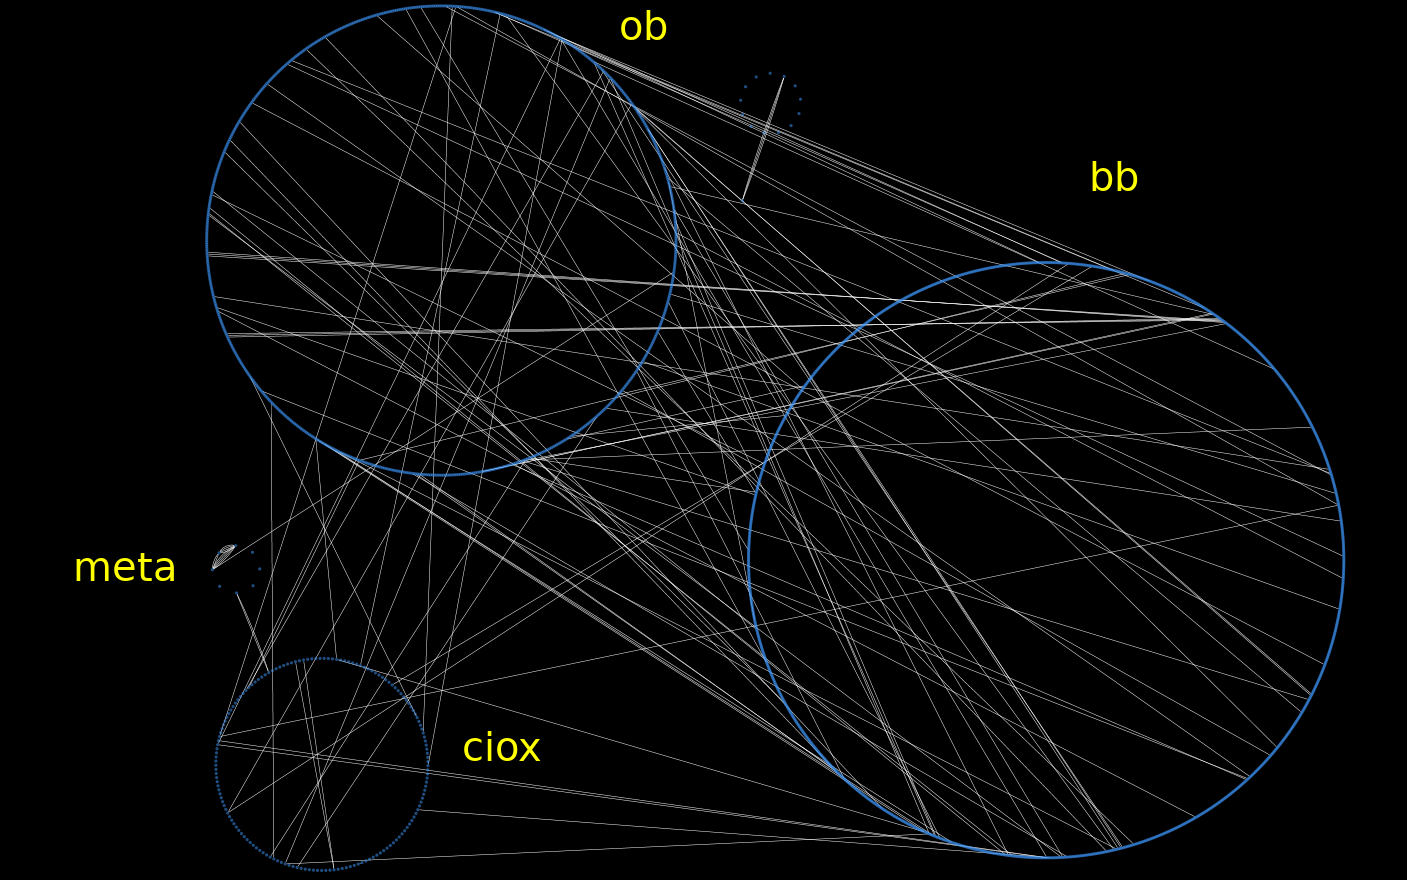
\includegraphics[width=\textwidth,height=\textheight,keepaspectratio]{img/types_classrelations_nosubclass_labelled.png}
\end{frame}

\begin{frame}{Cytoscape Desktop}
\centering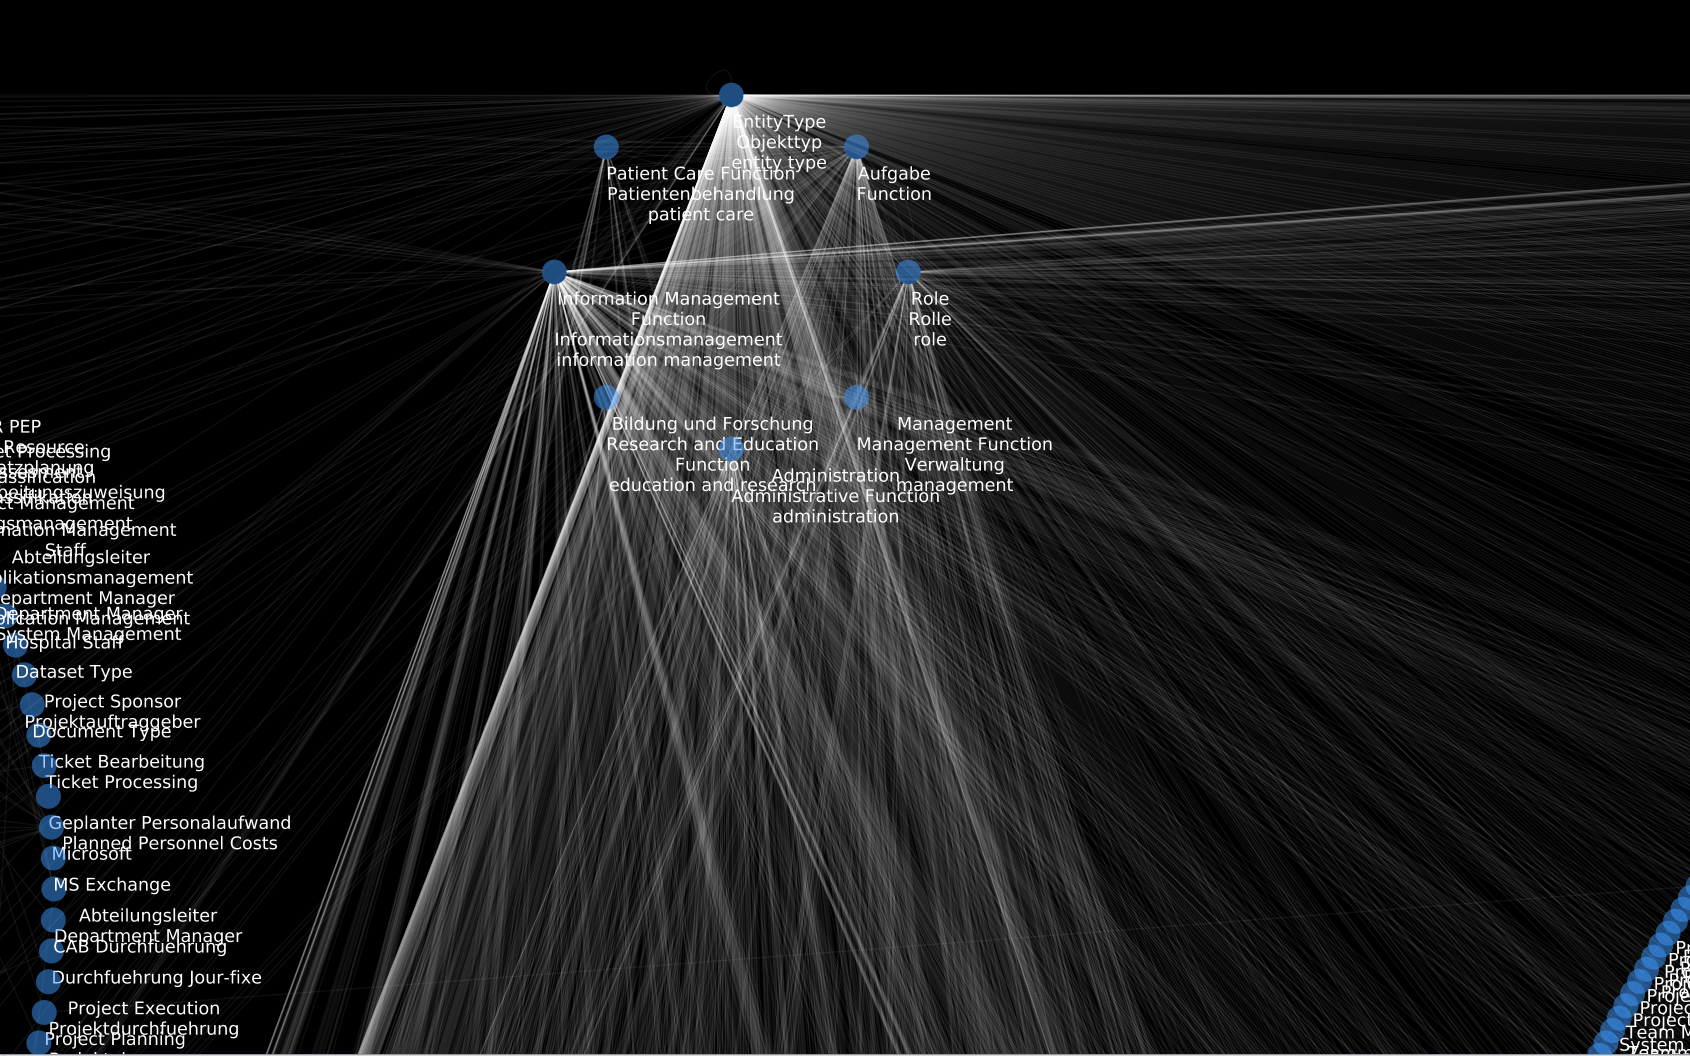
\includegraphics[width=\textwidth,height=\textheight,keepaspectratio]{img/types_classrelations_zoomed.png}
\end{frame}

\section{Nachträgliche Anmerkungen}

\begin{frame}{Diskussion}
\begin{itemize}
\only<1>
{
\item Transformation RDF->CSV mittels SPARQL Anatoli Zeiser beibringen
\item Visualisierung bereitet Einigen Kopfschmerzen, Option auf hellen Hintergrund gewünscht
\item Hervorheben von Interontologierelationen durch Filter (bereits erledigt)
\item Hinzufügen fehlender Daten im RDF-Browser
}
\only<2>
{
\item Beschriebene Prozesse stehen in der Mitte des Gesamtworkflows, Faktenextraktion ist davon unberührt.
\item Für zukünftige Extraktionen (z.B. durch Birgit Schneider) ändert sich also nicht direkt etwas.
\item Allerdings ist Änderung der Extraktion geplant, um großen Aufwand der Ontologiequalitätsverbesserung nach Extraktion zu verkleinern, durch Angleichen von Tabellenformular mit RDF und Ontologie.
\item Außerdem Untersuchung von Excel2OWL-Alternativen geplant.
}
\end{itemize}
\end{frame}

\begin{frame}{Referenzen und Weitere Informationen}
\begin{itemize}
\item \url{https://wiki.imise.uni-leipzig.de/Projekte/SNIK/ontologie/workflow}
\item \url{https://github.com/IMISE/snik-cytoscape.js}
\item \url{https://github.com/IMISE/snik-ontology} (URL wird evtl. geändert)
\item \url{https://bitbucket.org/imise/snik-ontology} (URL wird geändert)
\item \url{http://www.snik.eu/graph}
\item \url{http://www.snik.eu/pgraph}
\item \url{http://www.snik.eu/sparql}
\item \url{http://www.snik.eu/ontology}
\item Und natürlich \href{mich fragen}{mailto://konrad.hoeffner@imise.uni-leipzig.de} :-)
\end{itemize}
\end{frame}

\begin{frame}{Mitarbeit}
\begin{itemize}
\item alles open source (außer CIOx)
\item alle können sehr gerne Mitentwickeln
\item entweder pull-Request oder mich fragen und GitHub/Bitbucket-Account in Entwicklerteam aufnehmen lassen
\item readme-Dateien im Wurzelordner der Repositories lesen
\item Bug gefunden? Ticket im Repository erstellen.
\end{itemize}
\end{frame}

\end{document}
